%%%% ijcai24.tex

\typeout{IJCAI--24 Instructions for Authors}

% These are the instructions for authors for IJCAI-24.

\documentclass{article}
\pdfpagewidth=8.5in
\pdfpageheight=11in

% The file ijcai24.sty is a copy from ijcai22.sty
% The file ijcai22.sty is NOT the same as previous years'
\usepackage{ijcai24}

% Use the postscript times font!
\usepackage{times}
\usepackage{soul}
\usepackage{url}
\usepackage[hidelinks]{hyperref}
\usepackage[utf8]{inputenc}
\usepackage[small]{caption}
\usepackage{graphicx}
\usepackage{amsmath}
\usepackage{amsthm}
\usepackage{booktabs}
\usepackage{algorithm}
\usepackage{algorithmic}
\usepackage[switch]{lineno}
\usepackage{listings}
\usepackage{float}

\usepackage[
backend=biber
]{biblatex}


\addbibresource{bibliography.bib}

% Comment out this line in the camera-ready submission
% \linenumbers

\urlstyle{same}

% the following package is optional:
%\usepackage{latexsym}

% Following comment is from ijcai97-submit.tex:
% The preparation of these files was supported by Schlumberger Palo Alto
% Research, AT\&T Bell Laboratories, and Morgan Kaufmann Publishers.
% Shirley Jowell, of Morgan Kaufmann Publishers, and Peter F.
% Patel-Schneider, of AT\&T Bell Laboratories collaborated on their
% preparation.

% These instructions can be modified and used in other conferences as long
% as credit to the authors and supporting agencies is retained, this notice
% is not changed, and further modification or reuse is not restricted.
% Neither Shirley Jowell nor Peter F. Patel-Schneider can be listed as
% contacts for providing assistance without their prior permission.

% To use for other conferences, change references to files and the
% conference appropriate and use other authors, contacts, publishers, and
% organizations.
% Also change the deadline and address for returning papers and the length and
% page charge instructions.
% Put where the files are available in the appropriate places.


% PDF Info Is REQUIRED.

% Please leave this \pdfinfo block untouched both for the submission and
% Camera Ready Copy. Do not include Title and Author information in the pdfinfo section
\pdfinfo{
/TemplateVersion (IJCAI.2024.0)
}

\title{Knowledge Injection into Pretrained Language Models}


% Single author syntax
\author{
    Alexandre Domingues Andrade
    \affiliations
    Universidade de Coimbra
    \emails
    alexandrade@student.dei.uc.pt
}

\begin{document}

\maketitle

\section{Introduction}

Large Language Models (LLMs) have demonstrated remarkable capabilities in generating human-quality text, translating languages, and answering questions. However, their performance is critically dependent on the information provided in the input prompt. LLMs lack explicit memory of the vast datasets they were trained on;  their knowledge is implicitly encoded within their parameters, making accessing specific facts or ensuring consistency challenging. This presents a significant problem:  how to reliably and efficiently incorporate specific knowledge into an LLM's reasoning process, especially when dealing with tasks requiring precise factual recall or domain-specific expertise. Therefore, this work aims to investigate and evaluate practical methods for injecting knowledge into LLM prompts to improve the accuracy, reliability, and consistency of LLM-generated responses in general question-answering. It explores an approach involving structured knowledge bases, ultimately seeking to optimize the interaction between explicit knowledge and the inherent capabilities of the LLM. This work addresses multiple course topics, such as LLMs, LLMs Knowledge Injection, Entity Linking, and querying with SPARQL.

\section{Related Work}

The paper \textit{Knowledge-Augmented Language Model Prompting
for Zero-Shot Knowledge Graph Question Answering}\cite{baek2023knowledgeaugmentedlanguagemodelprompting} introduces a new methodology to input prompting enriched with knowledge graphs, named KAPING. Because this solution augments only the input, it does not require model training, thus completely zero-shot. Because it does not require training, any model can use it, close or open source, without pre-training or training the model for a specific task and dataset or even be used to enrich black-box algorithms hidden behind APIs (like ChatGPT).

This paper was conducted in a question-answering task, where questions are prompted to the LLM, and an answer is generated. The practicality of this input enrichment method is evident, as it can be seamlessly integrated into any question-answering bot or chat. The use of knowledge graphs, which are updated and accurate, overcomes the limitations of LLMs trained on static data.

The main steps described in the paper are as follows: The entities are extracted from the input. Then, the extracted entities are matched with the entities of the Knowledge Graph, and the triplets are extracted. Triples are transformed into text, and the sequence ranking is done to extract the k more relevant sentences to enrich the input. Finally, the triples and the question are fed to the LLM, and an answer is returned.

The framework was compared with multiple methods. No knowledge; that is just an answer generator without input enrichment. Randomly extracted knowledge, the input is enriched with random knowledge. Popular knowledge extraction, the triples are ranked by their popularity. The last method is Generated knowledge, which is extracted from other LLMs. The framework outperforms all LM prompting methods on zero-shot in Knowledge Graph Question Answering. In one of the experiments, the results using entities labelled in the dataset were compared with results when using the Entity Linking model ReFinED to extract the entities. As expected, the results with the entity linking model were worse than the labelled entities because of the model performance. The framework outperformed the other baseline methods by up to 48\% on average across multiple large language models of various sizes.

One limitation is the extraction of knowledge from multi-hop neighbourhoods. As stated in the paper, many times, the answer to the questions is outside the first-order neighbour, and it is necessary to retrieve 2-hop triples. The problem is that the quantity of triples grows exponentially when the order is raised; consequently, better triples ranking is needed.

\section{Data and Approach}

\subsection{Knowledge Database}

The source of the knowledge injected in the input prompts is Wikidata\cite{wikidata}. Wikidata is a collaborative, multilingual, free knowledge base that employs a structured data model based on the Resource Description Framework (RDF). It serves as a central repository of structured information, utilizing triples (subject-predicate-object) to represent knowledge. Each entity within Wikidata is identified by a unique identifier (QID), facilitating interlinking and semantic relationships between data points. This work retrieves data using two methods: querying the online endpoint with SPARQL queries and using a local JSON dump. In both, all claims/statements are retrieved for each identified entity. A Wikidata entity has the following structure:

\begin{lstlisting}
{
  "id": "Q60",
  "type": "item",
  "labels": {},
  "descriptions": {},
  "aliases": {},
  "claims": {},
  "sitelinks": {},
  "lastrevid": 195301613,
  "modified": "2020-02-10T12:42:02Z"
}
\end{lstlisting}

More details can be found in \cite{wikidata-structure}.

\subsection{Dataset}

The Natural Questions dataset is used to evaluate the algorithm \cite{natural-questions}. The Natural Questions dataset is a large-scale, publicly available dataset designed for training and evaluating question-answering (QA) systems that operate over unstructured text. Unlike many other QA datasets that utilize predefined question-answer pairs extracted from structured knowledge bases or carefully curated corpora, Natural Questions distinguishes itself by focusing on questions formulated naturally by real users of the Google Search engine. This characteristic introduces significant challenges that are not present in more artificial datasets.

The dataset comprises a collection of question-answer pairs derived from actual user queries submitted to Google Search. The corresponding answer is extracted from a Wikipedia page identified as relevant by Google's search algorithm for each question. Crucially, the answer extraction process is not constrained to a single sentence or paragraph; instead, it allows for selecting multiple sentences or spans of text that collectively comprise a comprehensive answer. This reflects the multifaceted nature of real-world questions, which often require more nuanced and extensive responses than those found in simpler QA datasets.

The dataset's structure includes:

\begin{itemize}
    \item Question: A natural language question posed by a user;
    \item Annotated Wikipedia Page:  The Wikipedia page deemed most relevant to the question;
    \item Long Answer:  A longer passage containing the answer, providing additional context.
    \item Short Answer:  A shorter, more concise answer extracted from the long answer.
\end{itemize}

The inherent complexity of Natural Questions stems from the inherent ambiguity and variability found in real user queries. Questions may be poorly phrased, contain implicit assumptions, or require complex reasoning for a satisfactory answer.

\subsection{Approach}

Injecting knowledge into prompts for Large Language Models (LLMs) requires bridging the semantic gap between unstructured textual input and structured knowledge bases. This process leverages entity linking, which identifies mentions of real-world entities (people, places, organizations, events, etc.) within the input text and maps them to corresponding entries in a knowledge base, such as Wikidata. This mapping is typically achieved by assigning unique identifiers (e.g., Wikidata IDs) to each recognized entity.

The algorithm retrieves related knowledge from the knowledge base by exploiting this structured information. This is often accomplished by traversing the knowledge graph, expanding outwards from the identified entity using a specified number of "hops" to define the neighbourhood size. The extracted knowledge, represented as triples (subject-predicate-object), is then transformed into a natural language format suitable for LLM input. A crucial filtering step is employed because this retrieved information often contains irrelevant details. This typically involves comparing each verbalized triple to the original question using a similarity metric (e.g., cosine similarity on sentence embeddings, lexical overlap) to assess relevance. Only the k* most relevant triples, where *k is a predefined parameter, are subsequently incorporated into the augmented prompt.

Finally, to evaluate the effectiveness of the knowledge injection, a similarity metric is applied to compare the generated answer with the ground truth answer. This assessment measures the degree to which the added knowledge contributes to a more accurate and comprehensive response, enabling a quantitative evaluation of the knowledge injection strategy's impact on LLM performance. This evaluation goes beyond simple accuracy metrics by considering the semantic relevance and meaningfulness of the knowledge injected concerningName "Tom Ayoola, Shubhi Tyagi, Joseph Fisher, Christos Christodoulopoulos, Andrea Pierleoni" has too many commas, skipping entry 'ayoola-etal-2022-refined' the question's context. The effectiveness of the knowledge injection is thus determined by its contribution to the quality and correctness of the LLM-generated answer, rather than solely on the presence of factual information.

\section{Implementation}

The high-level algorithm steps are:
\begin{enumerate}
    \item Load data from the dataset;
    \item Use entity-linking to retrieve the question entities;
    \item Get knowledge from the Wikidata
    \item Rank the knowledge obtained using similarity metrics
    \item Feed the knowledge and the question to a pre-trained language model (PLM)
    \item Compare the annotated answer with the output of the PLM
\end{enumerate}

\subsection{Dataset Loading}

The Natural Questions dataset is loaded using the HuggingFace library; for each dataset entry, the annotated question and answer are loaded into memory for subsequent processing.

\subsection{Entity linking}

Entity retrieval is performed using the ReFinED algorithm\cite{ayoola-etal-2022-refined}. This process yields the corresponding Wikidata IDs for each identified entity, which are subsequently used to retrieve relevant knowledge from the Wikidata knowledge base.


\subsection{Data Retrieval} \label{data-retrieval}

This work utilizes Wikidata as its primary source of structured information because it is a large-scale, general-purpose knowledge base. Two distinct data retrieval methods were employed: an online approach utilizing SPARQL queries against the publicly available Wikidata endpoint and an offline approach leveraging a local copy of the Wikidata JSON dump. Each method presents inherent trade-offs.

Then, for each entity, the neighbourhood space is explored, limited by the number of hopes; as mentioned in the approach, only k* more similar sentences go to the model. To evaluate the sentences, we used sentence transformers\cite{reimers-2019-sentence-bert} semantic textual similarity with the pre-trained model all-MiniLM-L6-v2.

Then, the neighbourhood space is explored for each entity, limited by the number of hopes. As the approach mentions, only k* more similar sentences go to the model. To evaluate the sentences, we used sentence transformers\cite{reimers-2019-sentence-bert} semantic textual similarity with the pre-trained model all-MiniLM-L6-v2.

The knowledge graph neighbourhood is explored for each identified entity, limited to a predefined number of hops. From this neighbourhood, only the k* most semantically similar sentences, as determined using sentence-BERT's all-MiniLM-L6-v2 model [Reimers and Gurevych, 2019], are selected for input to the language model.

While convenient, the online method has several limitations. Query timeouts frequently result in incomplete or corrupted data. Furthermore, shared computational resources at the endpoint and network latency constrain query throughput and data retrieval speed.

Conversely, utilizing a local Wikidata dump (approximately 1.6 TB uncompressed, but reduced to 200 GB through BTRFS filesystem compression), the offline method encounters limitations related to the host machine's hardware resources. While filesystem compression mitigates storage requirements, it introduces a significant performance bottleneck. On-the-fly decompression during data access substantially reduces retrieval speed, negating the expected performance gains of a local approach. While a non-compressed dump would eliminate this bottleneck, the available high-performance storage capacity (512 GiB) precludes this option. Future work may explore alternative storage solutions or optimized decompression techniques to address these limitations.

\subsection{Inference}

Following data retrieval, the retrieved knowledge and the question are provided as input to a pre-trained language model (PLM). Experiments utilized Llama 3\cite{grattafiori2024llama3herdmodels} versions 3.2, both 1 and 3 billion parameter variants. However, hardware limitations (8 GB VRAM) restricted the scope of experimentation, primarily focusing on the 1-billion parameter model. Given the objective of measuring answer improvement through external knowledge injection, the smaller model was deemed suitable. Its reduced parameter count and smaller context window provide a more pronounced opportunity to observe improvements resulting from adding factual information not present in the model's inherent knowledge.

\subsection{Metrics}

The same context similarity technique applied in \ref{data-retrieval} measures the impact of the knowledge prompted to the PLM. Still, the comparison is between the generated and ground truth answers here. The higher the similarity, the better.

\section{Experiments}

Different k and hop values were tested using the same questions to evaluate their impact.

\begin{figure}[h]
    \centering
    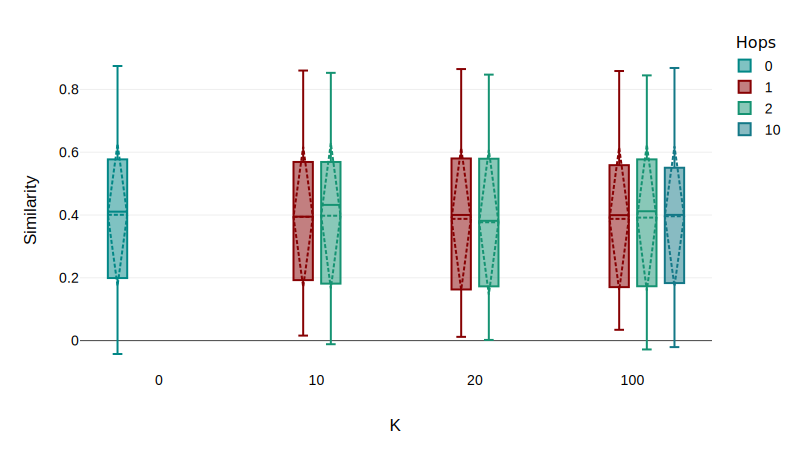
\includegraphics[width=1\linewidth]{results_llama1b.png}
    \caption{Llama 1B}
    \label{fig:results_llama1b}
\end{figure}

Figure \ref{fig:results_llama1b} shows that this knowledge injection method did not improve the Llama 3 model's answers on the NaturalQuestions dataset. Varying the neighbourhood size and a number of input sentences had no effect on the output. This is evident from the results for 0 hops and k=0, representing the model's output without knowledge injection.

\section{Discussion}

The dataset contains a variety of search queries submitted to Google, covering a broad range of topics. However, the structured data in Wikidata primarily focuses on established entities and historical facts. Consequently, many questions in the dataset cannot be answered using Wikidata alone. This is due to the incompleteness of Wikidata and the often nuanced and implicit references to entities within the natural language questions, some examples in \ref{tab:question}. In many situations, the entity extraction algorithm can not identify the entities. Thus, the context is not retrieved; this is evident when the entity's names are not written in capital letters. The following entities are all present in Wikidata, but the entity linking algorithm could not link the entities:

\begin{itemize}
    \item "what is andy's sisters name in toy story"
    \item "who made up the elf on the shelf"
    \item "when does season five of the killing come out"
\end{itemize}


\begin{table}[h]
    \begin{tabular}{p{1.5cm} p{3cm} p{3.4cm}}
        \toprule
         \textbf{Question}
         &\textbf{Ground Truth}
         &\textbf{Generated answer}\\
         \midrule
         what is the orange stuff on my sushi
         &tobiko
         &You're probably referring to tobiko or flying fish roe (also known as saba or fugu in Japanese). Tobiko is a type of edible roe that is commonly used as a garnish for sushi and sashimi.\\
         \hline
         who spread the theory that one is a product of the mind and body
         &René Descartes
         &The theory that one is a product of the mind and body is attributed to several ancient philosophers, but one of the most prominent is: René Descartes\\
         \hline
         what does the key to the city entitle you to
         &In some countries , such as the United States , an ornamental key -- the `` key to the city '' -- is presented to esteemed visitors , residents , or others whom the city wishes to honour . 
         &The "Key to the City" is a ceremonial honor bestowed upon an individual by the city they represent. The key itself is typically a symbol of the city's appreciation and recognition of the person's contributions, achievements, or service to the community.\\ 
    \end{tabular}
    \caption{Questions}
    \label{tab:question}
\end{table}

These results follow the ones presented in \cite{baek2023knowledgeaugmentedlanguagemodelprompting} for powerful models. Tables 1 and 5 in \cite{baek2023knowledgeaugmentedlanguagemodelprompting} reveal that for powerful models like GPT-3, the performance with knowledge injection is comparable to that without (No Knowledge). Furthermore, a comparison with the entity-linking results in Table 5 suggests that injecting knowledge into a robust model with entity-linking does not significantly improve answer generation. This indicates a potential limitation of simply injecting knowledge into strong language models.

Furthermore, the experiments revealed that increasing the neighbourhood size during knowledge retrieval did not yield improved results. While the system successfully retrieved information about individual entities mentioned in multi-entity questions, it struggled to capture the inter-entity relationships crucial for answering many complex queries. This highlights a critical gap in current approaches: the need for more effective reason over relational knowledge. To address this limitation, future work should explore more advanced knowledge graph traversal techniques, such as pathfinding algorithms. The successful implementation of such algorithms would necessitate using high-performance graph databases like Neo4j, enabling efficient querying and traversal of the complex relationships between entities. In summary, effectively integrating knowledge into LLMs requires addressing challenges in robust entity linking, developing sophisticated relational reasoning capabilities, and leveraging efficient graph database technologies.

\section{Conclusion}

This work investigated the efficacy of augmenting large language models (LLMs) with knowledge from Wikidata to enhance question-answering performance. The approach involved a multi-stage pipeline: entity linking to identify entities within input questions, knowledge retrieval from Wikidata using graph traversal, relevance filtering using semantic similarity, and finally, integrating the filtered knowledge into the LLM prompt. Experiments using the Natural Questions dataset and the Llama 3 (1B parameter) model revealed that this straightforward knowledge injection strategy did not significantly improve answer quality, as measured by semantic similarity to ground truth answers. 


\printbibliography

\end{document}

